\documentclass[]{itmo-student-thesis}

%% Опции пакета:
%% - specification - если есть, генерируется задание, иначе не генерируется
%% - annotation - если есть, генерируется аннотация, иначе не генерируется
%% - times - делает все шрифтом Times New Roman, требует пакета pscyr.

%% Делает запятую в формулах более интеллектуальной, например: 
%% $1,5x$ будет читаться как полтора икса, а не один запятая пять иксов. 
%% Однако если написать $1, 5x$, то все будет как прежде.
\usepackage{icomma}

%% Данные пакеты необязательны к использованию в бакалаврских/магистерских
%% Они нужны для иллюстративных целей
%% Начало
\usepackage{tikz}
\usetikzlibrary{arrows}
\usepackage{filecontents}
\begin{filecontents}{thesis.bib}
@article{ vyatkin-controllers,
  author      = {Yan, J. and Vyatkin, V.},
  title       = {Distributed Software Architecture Enabling Peer to Peer Communicating Controllers},
  journal     = {IEEE Transactions on Industrial Informatics},
  volume      = {9},
  number      = {4},
  year        = {2013},
  pages       = {2200-2209},
  langid      = {english}
}

@article{ deepmind-dqn-orig,
  author      = {Mnih, V. and others},
  title       = {Human-level control through deep reinforcement learning},
  journal     = {Nature},
  number      = {518},
  year        = {2015},
  pages       = {529-533},
  langid      = {english}
}

@article{ q-routing-orig,
  author      = {Boyan, J. A. and Littman, M. L.},
  title       = {Packet routing in dynamically changing networks: a reinforcement learning approach},
  journal     = {Advances in Neural Information Processing Systems},
  number      = {6},
  year        = {1994},
  pages       = {671-678},
  langid      = {english}
}

@article{ predictive-q-routing,
  author      = {Choi, S. P . M. and Yeung, D.-Y.},
  title       = {Predictive Q-Routing: A Memory-based Reinforcement Learning Approach to Adaptive Traffic Control},
  journal     = {Advances in Neural Information Processing Systems},
  number      = {8},
  year        = {1996},
  pages       = {945-951},
  langid      = {english}
}

@article{ dual-q-routing,
  author      = {Kumar, S. and Miikkulainen, R.},
  title       = {Dual reinforcement Q-routing: An on-line adaptive routing algorithm},
  journal     = {Artificial Neural Networks in Engineering},
  number      = {7},
  year        = {1997},
  pages       = {231-238},
  langid      = {english}
}

@phdthesis{ q-learning-orig,
    title    = {Learning from Delayed Rewards},
    school   = {King's College},
    address  = {Cambridge},
    author   = {Watking, C.},
    year     = {1989}
}

@article{ link-state-arpanet,
  author      = {McQuillan, J. M. and Richer, I. and Rosen, E. C.},
  title       = {The New Routing Algorithm for the ARPANet},
  journal     = {IEEE Trans. on Comm.},
  volume      = {28},
  number      = {5},
  year        = {1980},
  pages       = {711–719}
}

@article{ arpanet-orig,
  author      = {McQuillan, J. M. and Walden, D. C.},
  title       = {The ARPA network design decisions},
  journal     = {Computer Networks},
  volume      = {1},
  number      = {5},
  year        = {1977},
  pages       = {243-289}
}

@techreport{ rip-rfc,
  AUTHOR = {Hendrick, C.},
  TITLE = {Routing Information Protocol},
  TYPE= {RFC},
  NUMBER = {1058},
  YEAR = {1988},
  MONTH = {June},
}

@techreport{ ospf-rfc,
  AUTHOR = {Moy, J.},
  TITLE = {OSPF Version 2},
  TYPE = {RFC},
  NUMBER = 1058,
  YEAR = {1998},
  MONTH = {April},
}

@misc{ igrp-patent,
  title={Method and apparatus for routing communications among computer networks},
  author={Bosack, L.},
  url={https://www.google.com/patents/US5088032},
  year={1992},
  month=feb # "~11",
  publisher={Google Patents},
  note={US Patent 5,088,032}
}

@article{ bellman-ford,
  author = {Bellman, Richard},
  title = {On a routing problem},
  journal = {Quarterly of Applied Mathematics},
  number = {16},
  year = {1958},
  pages = {87-90}
}

@article{ dijkstra,
  author = {Dijkstra, E. W.},
  title = {A note on two problems in connexion with graphs},
  journal = {Numerische Mathematik},
  number = {1},
  year = {1959},
  pages = {269-271}
}

@article{ ali-nn-routing,
  author = {Ali, M. K. M. and Kamoun, F.},
  title = {Neural networks for shortest path computation and routing in computer
    networks},
  journal = {IEEE Transactions on Neural Networks},
  volume ={4},
  number = {6},
  year = {1993},
  pages = {941-953}
}

@article{araujo2001neural,
  title={A neural network for shortest path computation},
  author={Araujo, Filipe and Ribeiro, Bernardete and Rodrigues, Luis},
  journal={IEEE Transactions on Neural Networks},
  volume={12},
  number={5},
  pages={1067--1073},
  year={2001},
  publisher={IEEE}
}

@article{di1998antnet,
  title={AntNet: Distributed stigmergetic control for communications networks},
  author={Di Caro, Gianni and Dorigo, Marco},
  journal={Journal of Artificial Intelligence Research},
  volume={9},
  pages={317--365},
  year={1998}
}

@inproceedings{tan1993multi,
  title={Multi-agent reinforcement learning: Independent vs. cooperative agents},
  author={Tan, Ming},
  booktitle={Proceedings of the tenth international conference on machine learning},
  pages={330--337},
  year={1993}
}

\end{filecontents}
%% Конец

%% Указываем файл с библиографией.
\addbibresource{thesis.bib}

%% Всякая фигня
\DeclareMathOperator{\argmin}{argmin}
\DeclareMathOperator{\argmax}{argmax}

\begin{document}

\studygroup{M3438}
\title{Глубокие самообучающиеся агенты для мультиагентной системы маршрутизации}
\author{Мухутдинов Дмитрий Вадимович}{Мухутдинов Д.В.}
\supervisor{Фильченков Андрей Александрович}{Фильченков А.А.}{к.ф.-м.н}{доцент кафедры КТ}
\publishyear{2017}
%% Дата выдачи задания. Можно не указывать, тогда надо будет заполнить от руки.
\startdate{01}{сентября}{2016}
%% Срок сдачи студентом работы. Можно не указывать, тогда надо будет заполнить от руки.
\finishdate{31}{мая}{2017}
%% Дата защиты. Можно не указывать, тогда надо будет заполнить от руки.
%% \defencedate{15}{июня}{2015}

\addconsultant{Вяткин В.В.}{PhD, Luleå University of Technology}

%% Задание
%%% Техническое задание и исходные данные к работе
\technicalspec{
  Требуется разработать алгоритм решения обобщенной задачи маршрутизации, основанный на идее мультиагентного обучения нейронных сетей с подкреплением.
  Требуется применить метод к решению конкретных задач маршрутизации, таких как маршрутизация сетевых пакетов и управление конвейерной системой
  транспортировки багажа, и сравнить его c существующими алгоритмами.
}

%%% Содержание выпускной квалификационной работы (перечень подлежащих разработке вопросов)
\plannedcontents{
  \begin{enumerate}
  \item Обзор предметной области
  \item Реализация среды для эмуляции задачи сетевой маршрутизации
  \item Реализация среды для эмуляции конвейерной системы транспортировки багажа
  \item Разработка алгоритма маршрутизации на основе мультиагентного обучения нейронных сетей с подкреплением
  \item Реализация существующих алгоритмов решения задач маршрутизации
  \item Проведение экспериментов, интерпретация результатов
  \end{enumerate}
}

%%% Исходные материалы и пособия 
\plannedsources{\begin{enumerate}
    \item Richard S. Sutton and Andrew G. Barto. Reinforcement Learning: An Introduction. The MIT Press, 2012
    \item Mnih et al. Human-level control through deep reinforcement learning. Nature, 518(7540):529–533, 2015.
\end{enumerate}}

%%% Календарный план
\addstage{Ознакомление с предметной областью}{11.2016}
\addstage{Чтение статей, посвященных алгоритмам маршрутизации}{12.2016}
\addstage{Чтение статей, посвященных задаче обучения с подкреплением}{01.2017}
\addstage{Разработка сред для эмуляции задач маршрутизации}{03.2017}
\addstage{Разработка алгоритма маршрутизации, реализация существующих алгоритмов}{04.2017}
\addstage{Проведение экспериментов, написание пояснительной записки}{05.2017}

%%% Цель исследования
\researchaim{
  Разработка распределенного алгоритма решения задачи маршрутизации, подходящего для
  эффективного применения в различных условиях, включая киберфизические системы.
}

%%% Задачи, решаемые в ВКР
\researchtargets{\begin{enumerate}
    \item Формальная постановка обобщенной задачи маршрутизации.
    \item Разработка алгоритма решения поставленной задачи.
    \item Сравнение работы алгоритма с существующими решениями на практике.
\end{enumerate}}

%%% Использование современных пакетов компьютерных программ и технологий
\advancedtechnologyusage{
  Для решения задачи использовался язык программирования Python.
  При разработке систем эмуляции работы компьютерной сети и системы управления
  багажными конвейерами была использована библиотека Thespian. Для реализации и
  обучения нейронных сетей были использованы библиотеки TensorFlow и Keras.
}

%%% Краткая характеристика полученных результатов 
\researchsummary{
  Разработана формальная постановка обобщенной задачи маршрутизации в терминах
  мультиагентного обучения с подкреплением. Разработан алгоритм решения
  обобщенной задачи маршрутизации. Разработанный алгоритм по результатам
  экспериментов на практике не уступает современным специализированным
  алгоритмам решения задач сетевого роутинга и управления конвейерной системой,
  но благодаря обобщенной постановке задачи и применению нейронных
  сетей имеет широкий потенциал применения для решения задач, сводимых к задаче
  маршрутизации, в сложных условиях (таких, как киберфизические системы).
}

%%% Гранты, полученные при выполнении работы 
\researchfunding{
  При выполнении работы грантов получено не было.
}

%%% Наличие публикаций и выступлений на конференциях по теме выпускной работы
\researchpublications{
  По теме данной работы публикаций и выступлений на конференциях нет.
}

\graphicspath{{img/}}

%% Эта команда генерирует титульный лист и аннотацию.
\maketitle{Бакалавр}

%% Оглавление
\tableofcontents

%% Макрос для введения. Совместим со старым стилевиком.
\startprefacepage

Задача пакетной маршрутизации - это задача поиска кратчайшего пути в графе в условиях,
когда за каждый узел графа отвечает отдельный вычислительный процесс. Это
означает, что каждый отдельный узел графа должен принять решение о том, какому
из соседей следует отправить очередной пакет, чтобы тот достиг пункта назначения
как можно быстрее.

Задача пакетной маршрутизации впервые обрела актуальность с появлением
компьютерных сетей. Первые алгоритмы сетевой маршрутизации появились в процессе
разработки сети ARPANet. Именно тогда были изобретены такие подходы к пакетной
маршрутизации, как distance-vector\cite{arpanet-orig} и
link-state\cite{link-state-arpanet}, которые и по сей день лежат в основе таких
стандартных и широко применяемых алгоритмов сетевой маршрутизации, как Routing
Information Protocol (RIP)\cite{rip-rfc} и Open Shortest Path First (OSPF)\cite{ospf-rfc}.

Оба этих подхода основаны на идее вычисления кратчайшего пути между текущим
узлом сети и пунктом назначения пакета. Однако существуют и другие подходы к
решению задачи маршрутизации, основанные на идее обучения с подкреплением
(reinforcement learing). Первым таким алгоритмом стал алгоритм
Q-routing\cite{q-routing-orig}, основанный на методе
Q-learning\cite{q-learning-orig}. Этот алгоритм, как и его
модификации\cite{predictive-q-routing, dual-q-routing},
благодаря обучению с подкреплением оказался способен лучше адаптироваться к
изменениям в интенсивности сетевого трафика, чем алгоритмы, основанные на
вычислении кратчайшего пути, но из-за использования большего количества
служебных сообщений применение таких алгоритмов в реальных сетях ограничено.

Но стоит отметить, что задача маршрутизации встречается не только в компьютерных сетях, но
также и в более сложных средах, таких как киберфизические системы. Примером такой
задачи, частично решаемой с помощью алгоритмов маршрутизации, является
управление конвейерной системой (в частности, системой распределения багажа в
аэропорту). Задача управления такой системой в большинстве случаев решается с
помощью централизованных алгоритмов, и децентрализованное решение (основанное на
алгоритма Беллмана-Форда) было предложено совсем недавно\cite{vyatkin-controllers}. 
Такая задача отличается от задачи сетевого роутинга, с одной
стороны, тем, что служебные сообщения и целевые сообщения являются разными
сущностями (``целевое сообщение'' --- это чемодан, а служебные сообщения являются
цифровыми), и служебные сообщения передаются мгновенно по сравнению с целевыми.
С другой стороны, состояние каждого конвейера и всей системы в целом задается
большим количеством параметров --- такими как скорости конвейеров, положение,
количество и масса чемоданов на каждом конвейере, и так далее. С третьей
стороны, желательно, чтобы система оптимизировала не только скорость доставки
чемоданов до точки назначения, но и, к примеру, собственное энергопотребление.

Первое обстоятельство снимает технические ограничения на количество служебных
сообщений, что позволяет в полной мере применять алгоритмы на основе обучения с
подкреплением. Второе и третьи обстоятельства усложняют написание оптимального
детерминированного алгоритма и наталкивают на идею реализации приближенного
решения, например, с использованием нейронных сетей.

В настоящее время в области обучения с подкреплением с применением нейронных
сетей достигнуты впечатляющие успехи. Всплеск активности в этой области
произошел после выхода статьи команды Google DeepMind об обучении глубокой
сверточной нейронной сети игре на консоли Atari 2600\cite{deepmind-dqn-orig}.
Применению полученной модели к различным задачам в различных условиях посвящено
множество исследований, часть из них посвящена проблеме мультиагентного обучения
с подкреплением (multi-agent reinforcement learning). Так как задачу
маршрутизации можно сформулировать как задачу мультиагентного обучения с
подкреплением, имеет смысл применить данные наработки для ее решения.

В данной работе будет предложен алгоритм маршрутизации, основанный на методе
Q-routing, но использующий нейронную сеть в качестве обучающегося агента.
На данный момент не существует алгоритма маршрутизации, построенного по такому
принципу.

В главе 1 будет сформулирована обобщенная постановка задачи маршрутизации в
терминах мультиагентного обучения с подкреплением. Будут рассмотрены
существующие алгоритмы маршрутизации, их сильные и слабые стороны. Также будут
рассмотрены существующие методы обучения нейронных сетей с подкреплением, в том
числе в мультиагентном случае.

В главе 2 будет рассмотрен предложенный алгоритм и обоснованы решения, принятые
в ходе его разработки.

В главе 3 будут приведены экспериментальные результаты работы алгоритма для
задач пакетной маршрутизации в компьютерной сети и управления системой багажных
конвейеров. Будут приведены результаты работы в условиях неравномерной
нагрузки на сеть (или конвейерную систему) и изменения топологии сети. Также
будет проведено сравнение с существующими алгоритмами маршрутизации.

%% Начало содержательной части.
\chapter{Обзор предметной области}

\section{Постановка задачи}\label{task-setting}
Пусть задана сеть в виде графа: $G = (V, E)$. Каждому узлу и каждому ребру в сети
приписывается некоторое \textit{состояние}: узел v имеет состояние $s_v \in S_V$, ребро e
имеет состояние $s_e \in S_E$. Состояние всей сети, таким образом, описывается как
$s = (s_{v_1}, ... , s_{v_n}, s_{e_1}, ... , s_{e_m}) \in S$.

На узел сети $s \in V$ приходят пакеты $p = (d, prop)$, где $d \in V$ - узел
назначения пакета, а $prop$ - произвольная дополнительная информация о нем.
Обозначим множество всевозможных свойств пакета как $Prop$ ($prop \in Prop$), а
множество пакетов в целом, таким образом, как $P = (V, Prop)$. Также заданы
некоторые функции \textit{стоимости} прохождения данного пакета через ребра и
узлы сети, зависящие от их состояний:
$R_v : V \times S_V \times P \rightarrow \Bbb{R}^+$ - стоимость прохождения
пакета через узел, $R_e : E \times S_E \times P \rightarrow \Bbb{R}^+$. Мы явно
указываем, что стоимости неотрицательны, чтобы избежать таких постановок задач,
в которых существуют пути стоимости $-\infty$ (циклы отрицательной стоимости).

Задача пакетной маршрутизации заключается в том, чтобы определить, какому из
соседей $n \in \{v | (s, v) \in E\}$ узел $s$ должен перенаправить пакет
$p = (d, prop)$, чтобы ожидаемая стоимость пути от $s$ до $d$ была минимальной.

\section{Существующие алгоритмы маршрутизации}

Почти все существующие алгоритмы маршрутизации были разработаны для
маршрутизации пакетов в компьютерных сетях. Большинство алгоритмов маршрутизации
в компьютерных сетях, применяемых на практике, относятся к одному из двух
семейств алгоритмов --- дистанционно-векторные (distance-vector)\cite{arpanet-orig} или
состояния каналов связи (link-state)\cite{link-state-arpanet}.
Концептуально все алгоритмы внутри каждого из этих семейств одинаковы, и различаются только
техническими деталями реализации, обусловленными спецификой конкретной узкой
сферы применения. Поэтому мы не будем рассматривать алгоритмы каждого семейства
по отдельности, а рассмотрим только концепции в целом.

\subsection{Дистанционно-векторные алгоритмы}

Идея дистанционно-векторных алгоритмов (distance-vector algoritms) заключается в
следующем:

\begin{itemize}
\item Каждый маршрутизатор $s$ в сети хранит таблицу, в которой для каждого другого узла
  сети $d$ хранится следующая информация:
  \begin{itemize}
  \item Предполагаемое кратчайшее расстояние от $s$ до $d$
  \item Сосед $n$, которому нужно отправить пакет, чтобы пакет прошел по
    кратчайшему пути до узла $d$.
  \end{itemize}
\item Периодически каждый маршрутизатор рассылает свою версию таблицы кратчайших
  расстояний всем своим соседям
\item При получении вектора кратчайших расстояний от соседа маршрутизатор $s$
  сравнивает его поэлементно с текущей версией. Если оказывается, что наименьшая
  стоимость пути от соседа $n$ до узла $d$, сложенная c оценкой стоимости ребра
  $(s, d)$ меньше, чем наименьшая стоимость пути от $s$ до $d$ в текущей
  таблице, то значение в текущей таблице обновляется, и наилучшим соседом для
  отправки пакета в узел $d$ становится сосед $n$.
\end{itemize}

Как можно видеть, дистанционно-векторный алгоритм является, в сущности,
распределенной версией алгоритма Беллмана-Форда поиска кратчайшего пути в
графе\cite{bellman-ford}.

\begin{figure}[!h]
  \caption{Иллюстрация работы distance-vector алгоритма}\label{rip-img}
  \centering
  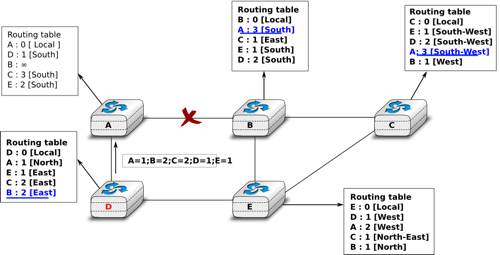
\includegraphics[scale=1.5]{dv-failure-2}
\end{figure}

Различные реализации дистанционно-векторного метода различаются, в частности,
оценками стоимости соединений в сети. Так, например, протокол RIP\cite{rip-rfc} просто
оценивает стоимость каждого соединения в 1, а IGRP\cite{igrp-patent} оценивает
стоимость соединений исходя из оценок задержки и пропускной способности.

Преимуществами дистанционно-векторных алгоритмов являются простота реализации и
низкие требования к памяти и вычислительной мощности. Недостатками же являются
низкая скорость распространения информации по сети и сложности с приспособлением
под изменяющуюся топологию (проблема count-to-infinity). Этих проблем
удается избежать при применении другого распространенного подхода - алгоритмов
на основе состояния канала связи. 

\subsection{Алгоритмы состояния канала связи}

В отличие от дистанционно-векторных алгоритмов, в алгоритмах состояния канала связи
(link-state) каждый узел сети хранит у себя модель всей сети в виде графа.
Рассмотрим шаги алгоритма подробнее:

\begin{itemize}
\item Каждый маршрутизатор периодически проверяет состояние соединений до
  соседей
\item При обнаружении обрыва какого-либо соединения алгоритм удаляет это
  соединение из собственного графа и рассылает соседям новую версию состояния
  соединений до них
\item Соседи обновляют собственные версии графов в соответствии с полученной
  информацией и пересылают сообщение дальше
\item Чтобы избежать зацикливания сообщений об обновлении состояния, каждое
  сообщение снабжается \textit{номером версии}. Маршрутизатор $n$ игнорирует
  сообщение от маршрутизатора $n$, если номер версии этого сообщения меньше или
  равен предыдущему.
\end{itemize}

\begin{figure}[!h]
  \caption{Иллюстрация работы link-state алгоритма}\label{ospf-img}
  \centering
  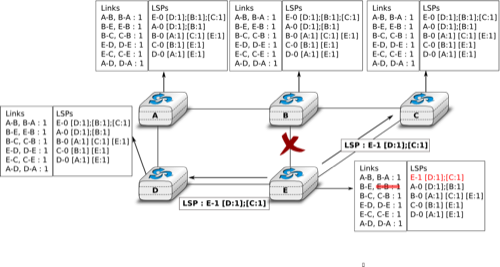
\includegraphics[scale=1.5]{ls-twoway}
\end{figure}

Имея информацию обо всей сети в целом, маршрутизатор может рассчитать кратчайшие
пути до всех остальных узлов. Обычно для этого используется алгоритм
Дейкстры\cite{dijkstra}. 

Link-state алгоритмы обладают способностью адаптироваться под изменения
топологии сети гораздо быстрее, чем distance-vector алгоритмы за счет
несколько более сложной реализации и чуть больших затрат по памяти и
вычислительной мощности. Это обуславливает то, что на данный момент именно
link-state протоколы, такие как OSPF\cite{ospf-rfc}, доминируют в сетевой
маршрутизации. Однако даже в решении задачи сетевой маршрутизации link-state
алгоритмы в чистом виде не лучшим образом адаптируются к повышению нагрузки в
сети. Рассматриваемые в дальнейшем другие алгоритмы, основанные на принципе
обучения с подкреплением, справляются с задачей адаптации к
изменчивой нагрузке лучше.

\subsection{Q-routing}\label{q-routing-desc}

Среди других подходов особый интерес представляют подходы на основе обучения с
подкреплением. Первым алгоритмом маршрутизации, основанным на этой идее, стал
алгоритм Q-routing\cite{q-routing-orig}. Принцип его работы таков:

\begin{itemize}
\item Каждый маршрутизатор $x$ хранит $Q_x(d, y)$ --- оценку минимального
  времени в пути до узла $d$, если следующим узлом на пути является сосед $y$.
  Очевидно, что $\forall y : Q_x(x, y) = 0$ 
\item Пакет, который необходимо доставить в узел $d$, отправляется соседу
  $y = \argmin\limits_{(x, y) \in E} Q_x(d, y)$
\item При получении пакета узел $y$ отправляет узлу $x$ время получения $t_r$ и
  собственную оценку оставшегося времени в пути
  $t = \min\limits_{(y, z) \in E} Q_y(d, z)$
\item Зная время отправления пакета $t_s$ и получив $t_r$ и $t$, узел $x$
  обновляет собственную оценку по формуле:
  $Q_x(d, y) = \alpha((t_r - t_s) + t - Q_x(d, y)) + Q_x(d, y)$,
  где $\alpha$ --- это learning rate, параметр алгоритма.
\end{itemize}

Было показано, что этот алгоритм способен хорошо адаптироваться к изменениям в
топологии сети и интенсивности трафика. Такие его модификации, как dual
Q-routing\cite{dual-q-routing} и predictive Q-routing\cite{predictive-q-routing}
демонстрируют еще более высокое качество маршрутизации. Однако по сравнению с
distance-vector или link-state методами данные алгоритмы используют гораздо
больше служебных сообщений (служебный пакет на каждую пересылку целевого
пакета), что ограничивает их применение в реальных высоконагруженных
компьютерных сетях.

Однако в задачах маршрутизации вне контекста компьютерных сетей это перестает
быть проблемой, так как целевые ``пакеты'' (чемоданы на конвейере, автомобили на
автостраде, etc.) и служебные сообщения в таких задачах являются объектами разной природы и
передаются по разным каналам, причем служебные сообщения по сравнению с целевыми
``пакетами'' доставляются мгновенно. Эти обстоятельства делают применение
алгоритмов обучения с подкреплением в таких задачах более привлекательным.

\subsection{Другие подходы}

Для полноты обзора приведем еще несколько примеров.

Идея использования нейросетей для решения задачи маршрутизации не нова. В
работах \cite{ali-nn-routing, araujo2001neural} для решения задачи поиска кратчайшего пути в графе
используются нейронные сети Хопфилда. Однако, эти исследования преследовали цель
ускорения вычисления кратчайшего пути за счет аппаратной реализации нейросети,
что кардинально отличается от цели текущей работы.

Еще одним интересным подходом является AntNet\cite{di1998antnet}. Это алгоритм,
построенный на идее исследования состояния сети с помощью специальных
пакетов-``агентов''. Алгоритм показал хорошие результаты в ходе исследований, но
не получил широкого применения, вероятно, в силу уже массового к тому времени
распространения link-state и distance-vector протоколов.

\subsection{Выводы по обзору существующих решений}

Все алгоритмы маршрутизации, рассмотренные в статье, были разработаны для
решения задачи маршрутизации именно в компьютерных сетях, но не для решения
задачи маршрутизации в общей формулировке. Таким образом, есть потребность в
разработке алгоритма, способного решать более общую задачу, что и является целью
данной работы.

\section{Применение обучения с подкреплением к задаче маршрутизации}

\subsection{Термины и понятия}

\textbf{Обучение с подкреплением} (reinforcement learning) --- вид машинного
обучения, в котором \textit{агент} (agent) каждый момент времени $t$
взаимодействует со \textit{средой} (environment), находящейся в
\textit{состоянии} (state) $s_t \in \mathcal{S}$ путем выбора
\textit{действия} (action) $a \in \mathcal{A}_{s_t}$ и получения
\textit{вознаграждения} (reward) $r_{t+1} \in \Bbb{R}$ c переходом в новое
\textit{состояние} $s_{t+1}$.

\begin{figure}[!h]
  \caption{Схема взаимодействия агента и среды в обучении с подкреплением}\label{rl-scheme}
  \centering
  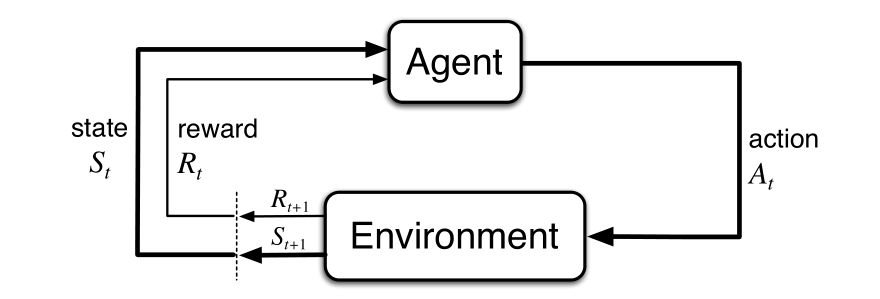
\includegraphics[scale=0.5]{rl-scheme}
\end{figure}

\textbf{Марковский процесс принятия решений} (Markov decision process, MDP) ---
это кортеж
$(\mathcal{S}, \mathcal{A}_s, P, R, \gamma)$, где

\begin{itemize}
\item $\mathcal{S}$ --- конечное множество состояний
\item $\mathcal{A}_s$ --- конечное множество действий, доступных из состояния
  $s$
\item $P(s' | s, a)$ --- вероятность того, что действие $a$ в состоянии $s$
  приведет к переходу в состояние $s'$ в следующий момент времени.
\item $R : \mathcal{S} \times \mathcal{A}_s \rightarrow \Bbb{R}$ ---
  вознаграждение за действия $a$ в состоянии $s$
\item $\gamma \in [0, 1]$ --- \textit{скидочный коэффициент} (discount factor),
  управляющий соотношением между важностью текущих вознаграждений и будущих вознаграждений.
\end{itemize}

\textbf{Оптимальной стратегией} для данного Марковского процесса принятия
решений называется такая функция выбора действий $\pi : \mathcal{S} \rightarrow \mathcal{A}_s$,
что взвешенная сумма вознаграждений $\sum\limits_{t=0}^{\infty} {\gamma^t
  R_{\pi(s_t)}(s_t, s_{t+1})}$ максимальна.

\textbf{Частично наблюдаемый Марковский процесс принятия решений} (Partially
observed Markov decision process, POMDP) --- это кортеж
$(\mathcal{S}, \mathcal{A}_s, P, R, \Omega, O, \gamma)$, где
\begin{itemize}
\item $\mathcal{S}$ --- конечное множество состояний
\item $\mathcal{A}_s$ --- конечное множество действий, доступных из состояния $s$
\item $P(s' | s, a)$ --- вероятность перехода из $s$ в $s'$ при выполнении
  действия $a$
\item $R : \mathcal{S} \times \mathcal{A}_s \rightarrow \Bbb{R}$ ---
  вознаграждение за действие $a$ в состоянии $s$.
\item $\Omega$ --- множество \textit{наблюдений}
\item $O(o | s', a)$ --- вероятность получения наблюдения $o$ при переходе в
  истинное состояние $s'$ в результате действия $a$. 
\end{itemize}

Определение оптимальной стратегии для частично наблюдаемого Марковского процесса
аналогично таковому для обычного.

Для Марковских процессов в условиях известности всех компонентов, включая $P$,
$R$ и $O$ существуют детерминированные методы нахождения оптимальной стратегии.
Однако найти оптимальную стратегию можно и в условиях неизвестности $P$, $R$ и $O$.

\textbf{Q-обучение} (Q-learning)\cite{q-learning-orig} --- это метод нахождения
оптимальной стратегии для Марковского процесса принятия решений, не требующий
информации о функции $R$ и распределении $P$. Метод заключается в оценке
\textit{функции полезности} (action-value function)
$Q(s,a)$. Функция полезности изменяется при каждом предпринятом действии $a$ с
переходом из состояния $s$ в $s'$ по следующей формуле:
\[
Q(s, a) = Q(s, a) + \alpha \left( r +
\gamma \cdot \max\limits_{a \in \mathcal{A}_{s'}} - Q(s', a) \right)
\]

Известно, что для любого конечного Марковского процесса принятия решений
Q-обучение находит оптимальную стратегию, т. е. $Q(s, a) \xrightarrow{t
  \rightarrow \infty} Q^*(s, a)$, и $\pi(s) = \argmax\limits_{a \in
  \mathcal{A}_s} {Q^*(s, a)}$ --- оптимальная стратегия.

\subsection{Формулировка задачи в терминах обучения с подкреплением}\label{rl-task-formulation}

К сожалению, сформулировать задачу маршрутизации в виде Марковского процесса
принятия решений довольно затруднительно. Попытаемся сформулировать ее
глобально. Пусть множество состояний $\mathcal{S}$ --- это Декартово произведение
состояний всех ребер и вершин в графе. Пусть также в состояние каждого ребра
(вершины) входит информация о всех пакетах, проходящих через это ребро
(обрабатывающихся в этой вершине). Пусть множество действий, доступных из
состояния $s \in \mathcal{S}$ $\mathcal{A}_s$ --- это множетво пар вида $(x,y)$,
где $x \in V$ --- это узел сети, имеющий в очереди пакет на обработку, а
$y \in \{V | (x, y) \in E\}$ --- один из его соседей. Таким образом, действие
интерпретируется как ``узел $x$ пересылает свой текущий пакет соседу $y$''.

К сожалению, у такой постановки задачи есть следующие проблемы:
\begin{enumerate}
\item Некоторые действия должны выполняться одновременно, а не одно за другим.
  Это можно формально обойти, сказав, что одновременно выполняющиеся действия
  $a_k, ... , a_{k+n}$ выполняются в последовательные моменты времени
  $t_k, ... , t_{k+n}$, либо изменив структуру множества действий
  $\mathcal{A}_s$: вместо пар $(x, y)$ рассматривать списки таких пар.
\item В любом случае невозможно узнать вознаграждение за действие $a_t$ сразу
  после перехода из состояния $s_t$ в $s_{t+1}$ --- вознаграждение за посылку
  пакета $p$ по ребру $e$ в вершину $v$ вычисляется как
  \[
  - \sum\limits_{t=t_k}^{t_{k+n}} {R_e(e, s_e^t, p)} -
  \sum\limits_{t=t_{k+n+1}}^{t_{k+m}} R_v(v, s_v^t, p)
  \]
  , где $t_k ... t_{k+n}$ --- моменты времени, в которые пакет проходил через
  ребро $e$, а $t_{k+n+1} ... t_{k+m}$ --- моменты времени, в которые пакет
  обрабатывался в узле $v$. (Суммы взяты с минусом, чтобы максимизация
  суммарного вознаграждения минимизировала суммарную стоимость путей пакетов).
  Это можно формально обойти, добавив в множество действий $\mathcal{A}_s$
  действия вида $a_e^p$ --- ``продолжить движение пакета
  $p$ по ребру $e$'' и $a_v^p$ --- ``продолжить продвижение пакета $p$ в очереди на
  обработку в узле $v$''. Однако такую формальную модель будет крайне сложно
  как-то применить на практике --- непонятно, как в какой-либо реальной задаче
  получить по отдельности стоимости вида $R_e(e, s_e^t, p)$ --- стоимости
  ``пребывания пакета $p$ на ребре $e$, которое находится в состоянии $s$.''
\end{enumerate}

Как можно видеть, несмотря на то, что формально процесс маршрутизации в сети
можно смоделировать как Марковский решающий процесс, оптимизация такой модели
представляет собой неподъемную задачу.

Гораздо более логичным кажется рассмотреть задачу с точки зрения отдельного
маршрутизатора как обучающегося агента. Используя подход \textit{независимого
  Q-обучения} (independent Q-learning, IQL)\cite{tan1993multi}, скажем, что
маршрутизатор считает всю остальную часть сети как среду, с которой он
взаимодействует. Безусловно, маршрутизатору недоступна исчерпывающая информация
о состоянии всей сети, а только небольшая ее часть --- свое собственное
состояние, и, возможно, какая-то еще информация (о соединениях с соседями, о
самих соседях, возможно, что-то еще). Таким образом, кажется, что работу такого
агента можно смоделировать как частично наблюдаемый Марковский процесс. Однако и
здесь мы встречаемся с проблемой не мгновенного получения вознаграждения --- к
тому времени, как агент узнает от среды (а именно --- от соседа, которому он
послал пакет) финальную стоимость прохождения пакета до соседа, он успеет
сменить множество состояний. Более того, в такой постановке задачи состояние
$s_{t+1}$ почти никак не зависит от действия $a_t$. К тому же такая постановка
мотивирует маршрутизатор все время посылать пакеты по ребру наименьшей
стоимости, максимизируя таким образом свой собственный выигрыш, что явно не
оптимизирует суммарную стоимость пути пакета.

Однако все встает на свои места, если мы сделаем формальный трюк и в качестве
агента, взаимодействующего со средой, рассмотрим \textit{пакет}, двигающийся в
сети и стремящийся минимизировать суммарную стоимость своего пути. Пакет
рассматривает всю сеть как среду, а наблюдаемое состояние маршрутизатора, в
котором он находится, включая идентификатор этого маршрутизатора, как
собственное \textit{наблюдение}  $o_t \in \Omega$. С точки зрения пакета, во время
его движения по ребру ничего не происходит --- внутри маршрутизатора пакет
выбирает действие $a_t \in \mathcal{A}_o$ --- одного из соседей, в которого нужно
перейти, ``мгновенно'' перемещается в этого соседа с получением вознаграждения $r_t$,
равного суммарной стоимости этого перемещения, взятого с отрицательным знаком, и
получает новое наблюдение $o_{t+1} \in \Omega$ --- состояние нового маршрутизатора.

Как можно видеть, в такой формулировке задача хорошо моделируется как частично
наблюдаемый Марковский процесс. Для нахождения оптимальной стратегии в частично
наблюдаемом Марковском процессе также можно использовать принцип Q-обучения.
Несмотря на то, что в общем случае в POMDP Q-обучение не сходится к оптимальной
стратегии, на практике это дает хорошие результаты.

Запишем формулу Q-обучения для поставленной задачи:

\[
Q(o_t, a_t) = Q(o_t, a_t) + \alpha \left( r_t +
\gamma \cdot \max\limits_{a \in \mathcal{A}_{o_{t+1}}} Q(o_{t+1}, a) \right)
\]

Заметим, что путь пакета конечен, и нас интересует оптимизация его полной
стоимости. Поэтому в данной задаче будем считать, что $\gamma = 1$.

Как можно видеть, если наблюдение состоит только из идентификатора текущего
узла, а вознаграждение является просто временем, потраченным пакетом на
перемещение, эта формула вырождается в формулу, используемую алгоритмом
Q-routing (\ref{q-routing-desc}). Безусловно, на практике, как и в оригинальном
алгоритме Q-routing, сам пакет не является агентом, вычисляющим собственную
стратегию. Вместо этого на место каждого очередного пакета себя ставит
маршрутизатор.

Как уже было замечено, в общем случае множество наблюдений $\Omega$ может быть
очень большим или даже бесконечным, что обуславливает необходимость
аппроксимации функции $Q(o, a)$. Для этого можно использовать нейросети. В
следующей главе будут рассмотрены примеры применения нейросетей в задачах
обучения с подкреплением.

\section{Обзор методов обучения нейросетей с подкреплением}

Активные исследования в области обучения с подкреплением с использованием
нейросетей начались c публикации командой DeepMind алгоритма
DQN\cite{deepmind-dqn-orig}. Алгоритм показал способность эффективно обучаться
игре в классические видеоигры на эмуляторе Atari 2600. 

Алгоритм DQN базируется на методе Q-обучения. В качестве состояния нейросеть
получает на вход текущее изображение игрового экрана. Набор действий
соответствует возможному набору игровых действий.

Ключевой проблемой при использовании Q-обучения с нейросетями является то, что
метод Q-обучения в применении к Марковским процессам с бесконечным числом
состояний, вообще говоря, не сходится к оптимальной стратегии. Алгоритм DQN
борется с этим обстоятельством с помощью experience
replay --- буферa из всех встреченных четверок $(s, a, r, s')$, где $s$ ---
начальное состояние, $a$ --- действие, предпринятое в этом состоянии, $r$ ---
полученное вознаграждение, $s'$ --- следующее состояние. Этот буфер работает как
``память'' нейросети: в каждый момент времени из буфера выбирается случайное
подмножество встреченных ситуаций, и нейросеть заново обучается на них,
``вспоминая'' игровой опыт.

\begin{figure}[!h]
  \caption{Устройство нейросети для приближения Q-функции}\label{dqn-scheme}
  \centering
  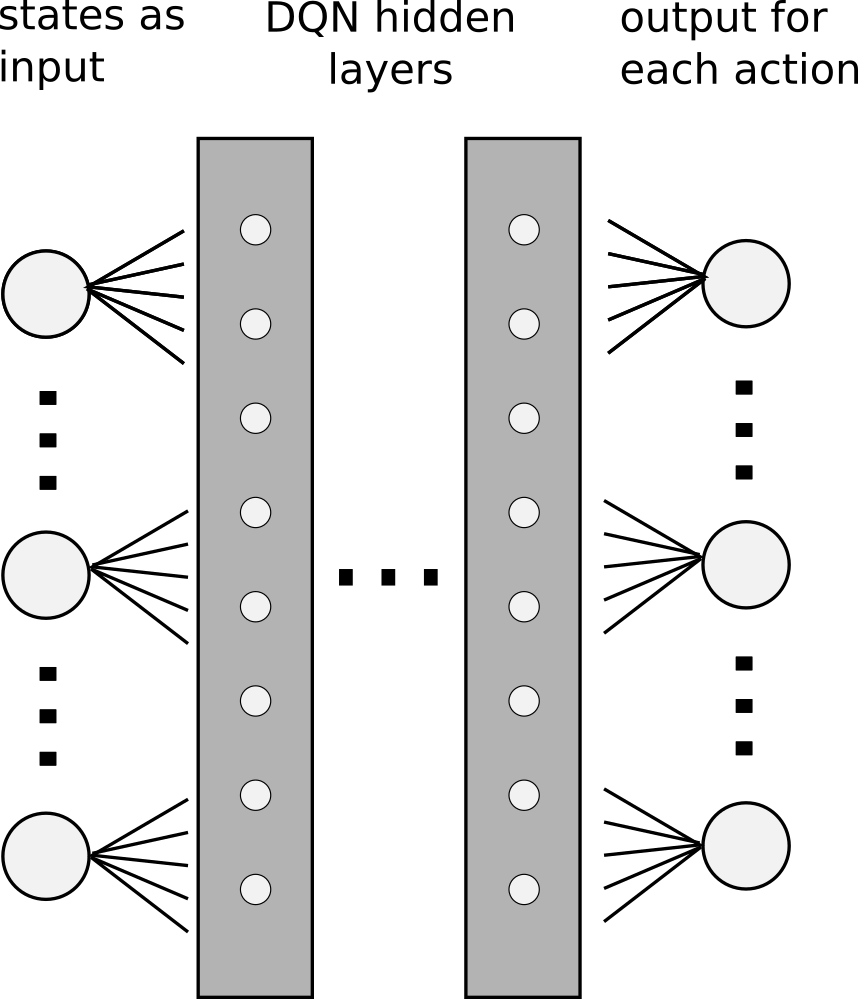
\includegraphics{dqn-scheme}
\end{figure}

TBD: закончить

\chapterconclusion

В главе 1 были рассмотрены существующие алгоритмы маршрутизации, их преимущества
и недостатки. Задача маршрутизации была сформулирована в терминах обучения с
подкреплением и были намечен подход к ее решению.

\chapter{Описание разработанного алгоритма}

Идея алгоритма заключается в объединении метода Q-routing\ref{q-routing-desc} с обучением
нейросетей. Однако очевидно, что простая замена табличной Q-функции на нейросеть
не даст положительных результатов. Чтобы использовать преимущества
нейросети, будут применены такие подходы, как \textit{предобучение} и
\textit{расширение наблюдаемого состояния}.

\section{Используемая архитектура нейросети}

Базовой частью любого текущего состояния $s$ (или, точнее \textit{наблюдения}
$o \in \Omega$ будем считать кортеж $(n, d, y_1 ... y_m)$, где $n$ --- это
идентификатор (номер) текущего узла, $d$ --- номер узла назначения текущего
пакета, а $y_1 ... y_m$ --- номера соседей текущего узла. Чтобы избежать
взаимозависимости оценок Q-функции для узлов с близкими номерами, будем
использовать \textit{унитарный код}, т. е. для сети с семью узлами номер 3 будет
кодироваться как 0010000, номер 5 --- как 0000100, и т. д. Для кодирования
множества соседей будем использовать тот же принцип, т. е. множество соседей 1,
3, 4 будет закодировано как 1011000. Таким образом, размер базового входного
состояния для нейросети составит $3n$, где $n$ --- количество узлов в сети.

Нейросеть имеет 2 скрытых полносвязных слоя с ReLU активаторами. Выходной слой
состоит из $n$ нейронов с линейными функциями активации, где $i$-ый нейрон
соответствует $i$-ому узлу в сети. К выходам узлов, не являющихся соседями
текущего, отдельно прибавляется $-\inf$ (на практике --- большое отрицательное
число, например -1000000). Таким образом, на выходе нейросети образуются оценки
функции $Q(s, a)$ для всех действий $a$, где для действий, недоступных в текущем
состоянии (узлов, не являющихся соседями), $Q(s, a) = -\inf$.

TBD: добавить иллюстрации

\section{Предобучение модели}
Как было указано в разделе \ref{rl-task-formulation}, мы будем моделировать
задачу маршрутизации как частично наблюдаемый Марковский процесс принятия
решений и рассматривать каждый пакет как независимого обучающегося агента,
взаимодействующего со средой. Однако такая постановка задачи неизбежно ведет к
нестационарности поведения среды по сразу двум причинам:

\begin{itemize}
\item Другие агенты, рассматриваемые как часть среды, тоже обучаются и меняют
  собственное поведение
\item Меняется характер трафика пакетов в сети
\end{itemize}

Нестационарность среды приводит к тому, что использование experience replay не
дает положительных результатов при обучении, так как прошлый опыт становится
неактуальным в новых условиях. Это приводит к тому, что процесс Q-обучения
перестает сходиться к оптимальному решению даже в случае равномерного
распределения трафика и низкой нагрузки. Чтобы частично справиться с этой
проблемой, будем использовать предварительное \textit{обучение с учителем}
(supervised learning). В качестве опорных данных будут использованы данные
работы алгоритма кратчайших путей в условиях низкой нагрузки и равномерно
распределенного трафика между узлами сети. В таких условиях алгоритм кратчайших
путей является оптимальным.

Здесь стоит заметить, что, вообще говоря, не во всех вариантах постановки задачи
маршрутизации можно вычислить стоимости прохождения пакета через ребра и узлы
сети даже в условиях низкой стационарной нагрузки. В таких случаях будем
довольствоваться некоторыми оптимистичными оценками на эти стоимости.

\section{Расширение наблюдаемого состояния}

Интуитивно понятно, что чем больше 

\chapter{Эксперименты}

TBD

%% Макрос для заключения. Совместим со старым стилевиком.
\startconclusionpage

TBD

\printmainbibliography

\end{document}
